\documentclass[8pt,a4paper,landscape]{extarticle}
% -- Layout ----
\usepackage[top=0.6cm, bottom=0.6cm, left=0.5cm, right=0.5cm, landscape]{geometry}

% -- Titles ----
\usepackage[
  tiny,                     % text size title
  compact                   % reduce vertical space before/after title
]{titlesec}
% \titlespacing*
\titleformat{\section}{\normalfont\small\bfseries}{\thesection}{0em}{} % Remove space before and after section titles
\titleformat{\subsection}{\normalfont\small\bfseries}{\thesubsection}{0em}{} % Remove space before and after subsection titles
\titlespacing*{\section}{0pt}{0pt}{0pt} % Remove space before/after section titles
\titlespacing*{\subsection}{0pt}{0pt}{0pt} % Remove space before/after subsec titles

% -- Colors ----
\usepackage[dvipsnames]{xcolor}
\definecolor{dmm}{RGB}{192,192,192} % Define a custom dimmed text color
\definecolor{cmt}{RGB}{61,123,123}

% -- Math ------
\usepackage{mathtools}
\usepackage{amssymb}
\usepackage{turnstile}%better vdash

% -- Lists -----
\usepackage[inline]{enumitem}
\setlist{noitemsep}% Remove vspace between items
% Set vspace before and after  list environments as well as the left margin
\setlist[itemize,1]{leftmargin=.6em,labelindent=0pt,labelsep=2pt,
  topsep=1pt,partopsep=1pt}
\setlist[enumerate,1]{leftmargin=1em,labelindent=0pt,labelsep=2pt,
  topsep=1pt,partopsep=1pt}
\setlist[itemize,2]{leftmargin=.3em,labelindent=1pt,topsep=1pt,partopsep=1pt}
\setlist[enumerate,2]{leftmargin=0.2em,labelindent=1pt,topsep=1pt,partopsep=1pt}
\setlist[description]{labelwidth=\linewidth,font=\small\bfseries,leftmargin=1em,topsep=1pt,partopsep=1pt}
% -- Code listing ---
\usepackage{listings}
\lstset{
  aboveskip=3pt,
  belowskip=3pt,
  basicstyle=\small\ttfamily,
  breaklines=true,
  % commentstyle=\upshape\ttfamily,
  captionpos=b,
  commentstyle=\color{cmt},
  columns=flexible,
  frame=single,
  keepspaces=false,
  keywordstyle=\bfseries,
  showspaces=false,
  showstringspaces=false,
  showtabs=false,
  tabsize=2,
}

% Parse Trees
\usepackage{tikz}
\usetikzlibrary{ arrows, automata, bbox, calc, positioning, tikzmark, decorations.pathmorphing, decorations.pathreplacing, decorations.shapes, }
\tikzset{
  >=stealth',
  node distance=1cm,
  recstate/.style={
    circle,draw=blue!50,fill=blue!20,thick,font=\small\sffamily,rounded corners=3pt,
    minimum size=1cm,inner sep=1pt
  },
  ivp/.style={draw,->,auto,font=\small\sffamily,bend angle=60},
  msi/.style={draw=Brown,->,auto,font=\small\sffamily,bend angle=80},
  msibs/.style={draw=RoyalBlue,->,auto,font=\small\sffamily,bend angle=80},
  msinl/.style={font=\footnotesize\sffamily}, %msi node label
  every edge/.style={draw,auto,font=\small\sffamily},
  every loop/.style={looseness=4},
  initial text=start,initial where=right
}

% Place a figure env right here via [H] option
\usepackage{float}

% Side by side figure
\usepackage{subcaption}
% \usepackage{caption}
% \captionsetup{belowskip=0pt, aboveskip=0pt}
\usepackage{pifont}

% -- Multi-Col layout --
\usepackage{multicol}

% No indentation
\setlength\parindent{0pt}
\setlength\abovedisplayskip{-5pt}
\setlength\belowdisplayskip{-5pt}
\setlength\abovedisplayshortskip{-4pt}
\setlength\belowdisplayshortskip{-4pt}
\setlength\tabcolsep{5pt}
\newcommand{\gor}{\;|\;}
\newcommand{\num}{\texttt{\#}~}
\newcommand{\pro}[1]{\textcolor{Brown}{#1}}
\newcommand{\bus}[1]{\textcolor{RoyalBlue}{#1}}
\renewcommand{\arraystretch}{1.2}


\begin{document}
% Suppress page number for all pages
\pagestyle{empty}

% Notes begin
\begin{multicols*}{3}
% \section*{Jargon}
\begin{itemize}
\item \textbf{synchronous iteration}: several processes start together at the beginning of each iteration and the next iteration must wait for all processors to finish current iteration, \textbf{L2P2}
\item \textbf{SPMD}: all UEs execute the same program (Single Program, SP) in parallel, but each has its own set of data (Multiple Data). In src code, usually a proc ID is used to uniquely label a UE
\item \textbf{Motivation} for parallelism (\textbf{L1P10}-\textbf{P11}):
  \begin{enumerate}
  \item speed/performance (1h vs 1w)
  \item tackle larger-scale problems
  \item keep power consumption and heat dissipation under control
  \item more $\cdots$ (see L1P11)
  \end{enumerate}
\item \textbf{Scales} of parallelism (\textbf{L1P12})
\item \textbf{peak flops/sec}$ = \# \text{cores} \times [\# \text{sockets}] \times \# \text{flops} \times \text{freq}$ (\textbf{L2-3P3})
\item ideal \textbf{speedup} is hard due to overheads (\textbf{L1P30})
  \begin{enumerate}
  \item idling (unbalanced load, sync, serial parts, etc)
  \item splitting computation into tasks
  \item communications among processes
  \end{enumerate}
\item \textbf{speedup}: $S_p = \frac{T_{seq}}{T_{par}} (\geq 1)$ (fixed problem size \textbf{L5P2})
\item \textbf{efficiency}: $E_p = \frac{S_{p}}{p} (0 < E_p \leq 1)$ (\textbf{L5P2})
\item \textbf{embarrassingly parallel}: problem solved without communication (\textbf{L5P3, L6P2})
\item \textbf{strong scalability}: fixed problem size + increasing $\# p \rightarrow$ perf. $\downarrow$
\item \textbf{weak scalability}: increasing $\# p$ and problem size $\rightarrow$ perf. $\downarrow$
\item \textbf{communication latency} time taken to communicate a message between 2 processors in a network
\item \textbf{minimal routing} takes 1 of shortest paths (XY-routing; E-cube)
\item \textbf{non-minimal} routing route the message along a longer path to avoid network congestion
\item \textbf{deterministic} routing determines a unique path \emph{solely} based on src and dest nodes
\item \textbf{adaptive} routing uses info on network state to determine message path (\textbf{L7P3})
\end{itemize}

% \section*{Amdahl's law (strong scaling law, \textbf{L5P5})}
\begin{equation}
  \label{eq:amdahl}
  S_p = \frac{T_{seq}}{T_{par}} = \frac{p}{pf + (1-f)} = \frac{1}{f + \frac{1-f}{p}}
\end{equation}
where $f$ is the serial portion that cannot be parallelized
\begin{tabular}{c|c}
  \hline
  \multicolumn{2}{l}{$S \rightarrow ? $ if run on 1000 CPU and 10\% ($f$) remains sequential} \\
  \hline
  $S_{ser} \quad p = 1$ & $S_{par} \quad p = 1000$  \\
  \hline
  2GFLOP/s  & $S_{ser} \times \frac{1}{0.1 + \frac{1-0.1}{1000}} \approx 9.91 \times S_{ser} = 19.82$ GFLOP/s \\
  \hline
\end{tabular}
\begin{tabular}{l|r}
  \hline
  \multicolumn{2}{l}{Calc $Ax=b$ where $A$ is $M \times N$ matrix} \\
  \multicolumn{2}{l}{$T_{ser} = 2MNT$ where $T$ is time for single float op} \\
  \multicolumn{2}{l}{$T_{sort} = 2M\log_2(M)T$ where sorting can only be sequential} \\
  \hline
  $T_{ser} \quad p = 1$ & $T_{par} \quad p = P \rightarrow \infty$ \\
  \hline
  $2MNT + 2M\log_2(M)T$ & $\frac{2MNT}{P} + 2M\log_2(M)T$ \\
  \hline
\end{tabular}
\begin{align*}
  S & = \frac{T_{ser}}{T_{par}} = \frac{2MNT + 2M\log_2(M)T}{\frac{2MNT}{P} + 2M\log_2(M)T} \\
    & = \frac{2MNT + 2M\log_2(M)T}{2M\log_2(M)T} \quad (P \rightarrow \infty \therefore \frac{2MNT}{P} \rightarrow 0) \\
    & = \frac{N}{\log_2(M)} + 1
\end{align*}
\section*{Gustafson's law (weak scaling law, \textbf{L5P7})}
\(S_p = p - f(p-1)\) where $f$ is the serial portion (independent of $p$ and problem size) and has the following assumptions:
\begin{enumerate}
\item the serial portion is kept constant when scaling problem size ($N$)
\item the perfectly parallelizable portion scales linearly with $\#p$ if $N$ scales linearly, then $T_{par}$ is kept constant.
\end{enumerate}

\section*{Moore's Law and Dennard Scaling (\textbf{L1P17})}

\begin{itemize}
  \item the two laws (\emph{underpin} exponential perf. increase of microprocessors)
  \item \textbf{Moore's} law (transistors doubles $\ne$ perf. doubles, \textbf{L1P17})
  \item \textbf{Dennard} Scaling (\textbf{L1P18-19}, examples below)
  \item[] $P = QfCV^{2}$ ($Q$: \# of transistors, $f$ frequency)
  \begin{tabular}{c|ccc}
    \hline
    \multicolumn{4}{l}{scale down feature size by  $\frac{1}{k}\approx 0.7$, then $k\approx 1.42, k^{2}\approx 2$} \\
    \hline
    & \# of trans. $Q$ & freq. $f$ & power usage $P$  \\
    \hline
    $Q_{0} = Q_{k}$ & unchanged & $f_k = k \cdot f_0$ & $P_k = (\frac{1}{k})P_0$\\
    $P_{0} = P_{k}$ & $Q_k = k^{2} \cdot Q_0$ & $f_k = k \cdot f_0$ & unchanged  \\
    \hline
    \multicolumn{4}{l}{feature size $\geq$ 100nm or $VI_{\text{leakage}}$  dominates power consumption} \\
    \hline
  \end{tabular}
\item these two also \emph{undermine} parallel computing however (\textbf{L1P21})
\item end of Dennard scaling $\rightarrow$ multicore era (\textbf{L1P23-24})
\end{itemize}

% \section*{Flynn's Taxonomy (\textbf{L2-3P12-14})}
\begin{tabular}{l|p{4cm}l}
  \hline
  Type & Note & Example \\
  \hline
  SISD & 1 ix process a stream data  & von Neumann model \\
  SIMD & 1 ix stream broadcast to many & vector processor; Quardrics\\
  MISD & no such machines  & - \\
  MIMD & each proc with its own ix/data & Gadi; most of top 500 \\
  \hline
\end{tabular}

% \section*{Store-and-Forward (SF) routing (\textbf{L7P5})}
\begin{equation*}
  t_{\text{comm}} = t_{s} + l(t_h + mt_w) \quad m \text{ is message size}; l \text{ is link num}
\end{equation*}
\begin{equation*}
  t_{\text{comm}} \approx t_{s} + lmt_w (\because t_h \ll mt_w \text{even for small} m)
\end{equation*}
\section*{Cut-Through (CT) routing (\textbf{L7P6})}
\begin{equation*}
  t_{\text{comm}} = t_{s} + lt_h + mt_w
\end{equation*}
If the communication is between nearest neighbors (that is, $l = 1$), or if the message size is small, then $T_{\text{comm}}$ is similar for store-and-forward and cut-through routing
\section*{One-to-all SF on different networks (\textbf{L7P9-10})}
\begin{tabular}{c|lc}
  \hline
  Network & Communication Cost & Source \\
  \hline
  Ring & $T_{\text{one-all}} = (t_s + t_{w}m) \frac{p}{2}$  & \textbf{L7P9} \\
  2D Mesh & $T_{\text{one-all}} = 2(t_s + t_{w}m) \frac{\sqrt{p}}{2}$ & \\
  3D Mesh & $T_{\text{one-all}} = 3(t_s + t_{w}m) \frac{\sqrt[3]{p}}{2}$ &  \\
  Hypercude & $T_{\text{one-all}} = (t_s + t_{w}m) \log_2 p$ & \textbf{L7P10} \\
  \hline
  \multicolumn{3}{l}{one-to-all broadcast with SF routing is \textbf{fastest} on hypercube}\\
  \hline
\end{tabular}
\section*{One-to-all CT on different networks (\textbf{L7P11-13})}
\begin{tabular}{c|l|c}
  \hline
  Network & Communication Cost & Source \\
  \hline
  Ring & $T_{\text{one-all}} = \log_2 p(t_s + mt_{w}) + t_h(p-1)$ & \textbf{L7P11} \\
  2D Mesh & $T_{\text{one-all}} = 2\log_2 (\sqrt{p})(t_s + mt_{w}) + 2t_h(\sqrt{p}-1) $ & \textbf{L7P12}\\
  Binary Tree & $T_{\text{one-all}} = \log_2(p)(t_s + mt_{w})+(\sum^{\log_2(p)}_{i=1}2i)t_h$ & \textbf{L7P13} \\
  \hline
  \multicolumn{3}{l}{one-to-all broadcast with CF does \emph{not} improve (not faster than SF)}\\
  \multicolumn{3}{l}{because of exclusively nearest-neighbor communication}\\
  \hline
\end{tabular}

\section*{All-to-All Store-and-Forward (SF) Routing (\textbf{L7P14-16})}
\begin{tabular}{c|l|c}
  \hline
  Network & Communication Cost & Source \\
  \hline
  Ring & $T_{\text{all-all}} = (p-1)(t_s + t_h mt_{w})$ & \textbf{L7P14} \\
  2D Torus & $T_{\text{all-all}} = 2(t_s + t_h)(\sqrt{p} - 1)+mt_{w}(p-1)$ & \textbf{L7P15}\\
  Hypercube & $T_{\text{all-all}} = 2\log_2(p)(t_s + t_h)+2(p-1)mt_w$ & \textbf{L7P16} \\
  \hline
\end{tabular}

\section*{Methods for containing interaction overheads}
\begin{enumerate}
\item Maximizing Data Locality
  \begin{itemize}
  \item Minimize Volume of Data-Exchange (minimize the overall volume of shared data, akin to maximizing the temporal data locality)
  \item Minimize Frequency of Interaction (there is a relatively high startup cost associated with each interaction on many architectures)
  \end{itemize}
\item Minimizing Contention and Hot Spots
\item Overlapping Computations with Interactions (init interaction early enough so that it's completed before it's needed for computation)
\item Replicating Data or Computations
\item Using Optimized Collective Interaction Operations
\item Overlapping Interactions with Other Interactions
\end{enumerate}
\section*{Parallel Algorithm Models}
\begin{itemize}
\item Data-Parallel (data parallelism, GPU) tasks are statically or semi-statically mapped onto processes and each task performs similar operations on different data
\item Task Graph: interrelationships among the tasks are utilized to promote locality or to reduce interaction costs; typically employed to solve problems in which the amount of data associated with the tasks is large relative to the amount of computation associated with them.
\item Work Pool: a dynamic mapping of tasks onto processes for load balancing in which any task may potentially be performed by any process; no desired premapping of tasks onto processes
\item Master-Slave (manager-worker): one or more master processes generate work and allocate it to worker processes
\item Pipeline or Producer-Consumer: a stream of data is passed on through a succession of processes, each of which perform some task on it
\end{itemize}

% \section*{Matrices Multiplication (Square n $\times$ n)}
\begin{equation*}
  A_{n,n} \times B_{n,n} =
 \begin{bmatrix}
  a_{11} & a_{12} & \cdots & a_{1n} \\
  a_{21} & a_{22} & \cdots & a_{2n} \\
  \vdots  & \vdots  & \ddots & \vdots  \\
  a_{n1} & a_{n2} & \cdots & a_{nn}
 \end{bmatrix}
  \begin{bmatrix}
  b_{11} & b_{12} & \cdots & b_{1n} \\
  b_{21} & b_{22} & \cdots & b_{2n} \\
  \vdots  & \vdots  & \ddots & \vdots  \\
  b_{n1} & b_{n2} & \cdots & b_{nn}
 \end{bmatrix}
\end{equation*}
\begin{align*}
  \label{eq:mmitem}
  C_{ij} & =  \begin{bmatrix}
                a_{i1} \\
                a_{i2} \\
                \vdots \\
                a_{in}
              \end{bmatrix}
              \begin{bmatrix}
                b_{1j} & b_{2j} & \cdots & b_{nj}
              \end{bmatrix} =
           \begin{bmatrix}
                a_{i1} \\
                a_{i2} \\
                \vdots \\
                a_{in}
           \end{bmatrix}
           \cdot
           \begin{bmatrix}
                b_{1j} \\
                b_{2j} \\
                \vdots \\
                b_{nj}
           \end{bmatrix} \\
         & = a_{i1}\cdot b_{1j}+a_{i2}\cdot b_{2j}+\cdots+a_{in}\cdot b_{nj} \\
         & = \sum_{i,j=1}^{n}a_{ij}\cdot b_{ji}
\end{align*}

\lstinputlisting[language=C,linerange={4-17}]{sec/matrixmul1.c}

% \section*{Overhead and resolution of timer}
\begin{itemize}
\item Timer \emph{overhead} is the amount of time it takes to call the timer function
\item Usually to measure the overhead for $n$ times and calc. the average
\item[] $T_{\text{overhead}} = \text{Average}(\text{overhead}_1,\text{overhead}_2,\cdots,\text{overhead}_n)$
\item The total time to run a program will be increased by $T_{\text{ overhead}} * m$ where $m$ is the number of times the timer is called
\item Timer \emph{resolution} is the period of time below which the timer will sometimes report a value of zero
\item[] $T_{\text{res}} = \texttt{MPI\_Wtime()/*end*/} - \texttt{MPI\_Wtime()/*start*/}$ (of type \texttt{double})
\item \texttt{MPI\_Wtick()} also gives the time resolution (of type \texttt{double})
\item The latency is the time to send an empty message but in some cases the smallest-sized message can be used to that end
\end{itemize}

% \section*{Roofline Model (naive)}
\begin{minipage}{.6\linewidth}
  \flushleft
  \begin{itemize}
  \item max task-processing speed: \textcolor{red}{$P$ [flop/s]}
  \item bottleneck
    \begin{itemize}[label=-]
    \item execution of work: P$_{peak}$ [flop/s]
    \item data path: \textcolor{Green}{$I\cdot b_s$} [flop/byte $\cdot$ byte/s]
    \end{itemize}
  \end{itemize}
\[
\textcolor{red}{P} = \textsf{min}(\textcolor{Cyan}{P_{\text{peak}}}, \textcolor{Green}{I\cdot b_{s}})
\]
  \begin{itemize}
  \item High intensity: P limited by execution
  \item Low intensity: P limited by data transfer
  \item best use of resources (also max use of power): \textcolor{Tan}{Knee} at $P_{max} = I \cdot b_s$
  \item \textcolor{red}{roofline} is ``optimistic'' because it assumes data moves at \textcolor{red}{light speed}
  \end{itemize}
\end{minipage}
\begin{minipage}{.4\linewidth}
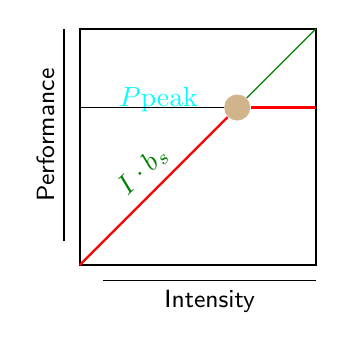
\begin{tikzpicture}
  % Knee
  \node[shape=circle,radius=1mm,fill=Tan]
  (knee) at (2,2) {};

  % Peaknode
  \node[color=Cyan] (peak) at (1,2.1) {$P\text{peak}$};

  % Ibsnode
  \node[color=Green,rotate=45] (ibs) at (.8,1.2)
  {$I\cdot b_s$};

  % rectangle coordinates
  \draw[thick] (0,0) rectangle (3,3);

  % y axis
  \draw (-.2, .3) edge[]
  node[above,sloped]{Performance} (-.2,3);

  % x axis
  \draw (.3, -.2) edge[]
  node[below]{Intensity} (3,-.2);

  % Peak
  \draw (0,2) -- (knee);
  \draw[color=red,thick] (knee) -- (3,2);

  % AI (I * Bs)
  \draw[color=red,thick] (0,0) -- (knee);
  \draw[color=Green] (knee) -- (3,3);

\end{tikzpicture}
\end{minipage}

\section*{MPI}
Message-passing programming paradigm has 2 key attributes:
\begin{enumerate}
\item partitioned address space (not shared), which implies
  \begin{itemize}
  \item each data element must belong to 1 partitioned space
  \item interactions (read-only/read-write) require coop of 2 procs
  \end{itemize}
\item supports only \emph{explicit} parallelization
\end{enumerate}
Two common causes of \textbf{deadlock} in MPI:
\begin{enumerate}
\item false order or \texttt{send} and \texttt{recv}
\item system send-buffer fill-up
\end{enumerate}

\subsection*{Starting and terminating MPI}
\begin{minipage}{0.5\linewidth}
  \begin{itemize}
  \item All the following snippets have a surrounding pair of \texttt{MPI\_Init} and \texttt{MPI\_Finalize}.
  \item After \texttt{MPI\_Finalize}, even another \texttt{MPI\_Init} is \emph{not} allowed.
  \item Both \texttt{Init} and \texttt{Finalize} must be called by all processes.
  \item In the end, \texttt{MPI\_SUCCESS} returned if nothing goes wrong.
  \end{itemize}
\end{minipage}
\begin{minipage}{0.48\linewidth}
\begin{lstlisting}[language=c,xleftmargin=1pt]
// argc, argv from main
// No MPI calls can be here
MPI_Init(&argc, &argv);
// parallel computation
// .
// .
// .
// commu betwn procs
MPI_Finalize();
// No MPI calls can be here
\end{lstlisting}
\end{minipage}

\subsection*{Getting information}
\begin{minipage}{0.5\linewidth}
  \flushleft
  \begin{itemize}
  \item Each proc will call these two fns to get the info for comm.
  \item Output vars are \texttt{size} and \texttt{rank}.
  \item \texttt{size}/\texttt{rank} can be declared before \texttt{Init}.
  \item \textbf{in} args are passed to MPI fns
  \item \textbf{out} args will be assigned values.
  \item \textbf{in}/\textbf{out} args must be declared before any usage.
  \end{itemize}
\end{minipage}
\begin{minipage}{0.48\linewidth}
\begin{lstlisting}[language=c,xleftmargin=1pt]
// before any MPI comm
// get how many processors
int size; // or world_size
MPI_Comm_size(MPI_COMM_WORLD, &size);

// get the current proc rank
int myrank;
MPI_Comm_rank(MPI_COMM_WORLD, &myrank);
\end{lstlisting}
\end{minipage}

\subsection*{Sending and receiving messages (blocking commu)}
\begin{itemize}
\item commonly used for point-to-point communications.
\item blocking send blocks until msg gets copied out of the send buffer (either into a system buffer at src process or sent to dest process)
\item blocking recv returns only after msg gets received and copied into the recv buffer
\end{itemize}
\begin{lstlisting}[language=c]
// MPI defined const MPI_TAG_UB with guaranteed range [0,32767]
// data of type dt will be stored in `buf' (consecutive in mem)
// `buf' len is specified by `count'
int MPI_Send(void *buf,            /* in, data buffer  */
             int count,            /* in, data count   */
             MPI_Datatype dt,      /* in, data type    */
             int dest,             /* in, dest rank    */
             int tag,              /* in, msg type tag */
             MPI_Comm, comm        /* in, communicator */
);

// Recv can accept at most count data otherwise overflow
// with MPI_ERR_TRUNCATE.  So Recv needs not know the
// exact size of messages being sent
int MPI_Recv(void *buf,            /* out,data buffer  */
             int count,            /* in, data count   */
             MPI_Datatype dt,      /* in, data type    */
             int source,           /* in, source rank  */
             int tag,              /* in, msg type tag */
             MPI_Comm comm,        /* in, communicator */
             MPI_Status *status    /* out, recv status */
);
\end{lstlisting}
\subsection*{Non-blocking communication}
\begin{itemize}
\item commonly used to overlap communications with computation.
\item need appropriate hardware support.
\item \texttt{MPI\_Isend} returns before data copied out of the buffer.
\item \texttt{MPI\_Irecv} returns before data received and copied into the buffer.
\item later in the program, must check if send/recv is complete.
\item \texttt{MPI\_Irecv} not take \texttt{status} arg
\item \texttt{status} of recv is returned by \texttt{Test}/\texttt{Wait}
\item \texttt{req} (non-blocking) is different than \texttt{status} (blocking).
\item \texttt{req} is also returned by \texttt{MPI\_Test} and \texttt{MPI\_Wait}
\item \texttt{MPI\_Wait} until a non-blocking operation actually finishes.
\end{itemize}
\begin{lstlisting}[language=c]
// ISend returns immediately w/t blocking current proc
// Sending goes on in the background and later the proc
// must Wait/Test for completion of sending.  Only after
// that it's safe to reuse the `buf' (to overwrite it)
int MPI_Isend(void *buf,           /* in, data buffer  */
             int count,            /* in, data count   */
             MPI_Datatype dt,      /* in, data type    */
             int dest,             /* in, dest rank    */
             int tag,              /* in, msg type tag */
             MPI_Comm comm,        /* in, communicator */
             MPI_Request *req,     /* out,handler      */
);

// Irecv returns immediately w/t blocking current proc
// Receiving goes on in the background and later the proc
// must Wait/Test for completion of receiving.  Only after
// that it's safe to use received data (to compute)
// NOTE: no status arg needed for non-blocking Irecv
// status is returned by MPI_Test and MPI_Wait instead
int MPI_Irecv(void *buf,           /* out,data buffer  */
             int count,            /* in, data count   */
             MPI_Datatype dt,      /* in, data type    */
             int source,           /* in, source rank  */
             int tag,              /* in, msg type tag */
             MPI_Comm comm,        /* in, communicator */
             MPI_Request *req      /* out,handler      */
);
\end{lstlisting}

% \subsection*{MPI Test and Wait}
\begin{minipage}{0.5\linewidth}
\begin{lstlisting}[language=c,xrightmargin=2pt]
// test if a non-blocking
// operation has finished
// this fn is non-blocking
int MPI_Test(
 MPI_Request *request,/*in */
 int *flag,           /*out*/
 MPI_Status *status   /*out*/
);

// this fn is blocking
// it will return only when
// request indicates finish
int MPI_Wait(
 MPI_Request *request,/*in */
 MPI_Status *status   /*out*/
);
// Ok to Isend with blk Recv
\end{lstlisting}
\end{minipage}
\begin{minipage}{0.5\linewidth}
  \flushleft
  \begin{enumerate}[leftmargin=.8em]
  \item if a non-blocking op finished
    \begin{itemize}
    \item allowed periodical checking for completion
    \item \texttt{flag} set to \texttt{true} (non-zero in C)
    \item request object deallocated
    \item \texttt{*request} $\rightarrow$ \texttt{MPI\_REQUEST\_NULL}
    \item \texttt{status} object gets info about op
    \end{itemize}
  \item if a non-blocking op not finished
    \begin{itemize}
    \item \texttt{flag} set to \texttt{false} (zero in C)
    \item \texttt{*request} not modified
    \item \texttt{status} undefined
    \item \texttt{MPI\_Wait} blocks until \texttt{*request} indicates finish (see 1)
    \end{itemize}
  \item mix of blk \& non-blk is OK
  \end{enumerate}
\end{minipage}

\subsection*{Collective Communication \& Computation}
\begin{itemize}
\item Collective comm typically outperforms point-to-point comm
\item Code becomes more compact and easier to read
\item All collective comm fns in MPI take a communicator arg that defines the group of procs participating in the collective operation
\item All the procs belonging to this communicator participate in the op
\item All of them \textbf{must} call the collective comm fns (see below)
\item Collective comm ops \emph{do not} act like barriers (a proc could go past its call for the collective communication operation, even before other processes have reached it)
\item Collective comm ops acts like a \emph{virtual} sync step (no need for tags)
\item All procs in group (communicator) must specify same src-/target-proc
\item For most collective comm ops, MPI provides two different variants:
  \begin{enumerate}
  \item transfers equal-size data to or from each process
  \item transfers data that can be of different sizes
  \end{enumerate}
\end{itemize}

% Barrier
% \subsection*{Barrier}
\begin{minipage}{0.5\linewidth}
  \flushleft
  \begin{itemize}
  \item only arg is communicator
  \item returns only after all procs in group have called this fn
  \end{itemize}
\end{minipage}
\begin{minipage}{0.5\linewidth}
\begin{lstlisting}[language=c,xleftmargin=1pt]
// comm defines the group
// of procs that are synced
int MPI_Test(MPI_Comm comm);
\end{lstlisting}
\end{minipage}

% Broadcast
% \subsection*{Broadcast}
\begin{minipage}{0.5\linewidth}
  \flushleft
  \begin{itemize}
  \item only arg is communicator
  \item returns only after all procs in group have called this fn
  \item data stored in root (aka. src) buf
  \item data totaling count entries of \texttt{dt}
  \item root data amount \texttt{==} amount recv by each proc
  \item \texttt{count} and \texttt{dt} fields must match on all procs
  \end{itemize}
\end{minipage}
\begin{minipage}{0.5\linewidth}
\begin{lstlisting}[language=c,xleftmargin=1pt]
// for root, data goes out
// for others, data comes in
int MPI_Bcast(
  void *buf,       /*inout*/
  int count,       /*in   */
  MPI_Datatype dt, /*in   */
  int root,        /*in   */
  MPI_Comm comm    /*in   */
);
// each proc gets same data
\end{lstlisting}
\end{minipage}

\begin{minipage}{0.5\linewidth}
  \flushleft
  \begin{itemize}
  \item src (aka. root) proc sends a diff. part of \texttt{sendbuf} to each procs, including itself
  \item received data stored in \texttt{recvbuf}
  \item proc $i$ recv \texttt{sendcount} contiguous \texttt{senddt} eles from $i*\texttt{sendcount}$ location of \texttt{sendbuf} of src proc
  \item assume that \texttt{senddt* sendbuf}
  \item \texttt{MPI\_Scatter} must be called by all procs with same vals for the \texttt{sendcount}, \texttt{senddt}, \texttt{recvcount}, \texttt{recvdt}, \texttt{source}, and \texttt{comm} args
  \item \texttt{sendcount} is $\#$ elements sent to each individual procs.
  \end{itemize}
\end{minipage}
\begin{minipage}{0.5\linewidth}
\begin{lstlisting}[language=c,xleftmargin=1pt]
// source is the root proc
// root sends parts of data
// to all procs  + itself
int MPI_Scatter(
  void *sendbuf,      // in
  int sendcount,      // in
  MPI_Datatype senddt,// in
  void *recvbuf,      // out
  int recvcount,      // in
  MPI_Datatype recvdt,// in
  int source,         // in
  MPI_Comm comm       // in
);
// each proc gets diff data
// it's usually the case:
// sendcnt = sendbuf.len / p
\end{lstlisting}
\end{minipage}

% Gather
\begin{minipage}{0.5\linewidth}
  \flushleft
  \begin{itemize}
  \item with $p$ procs in \texttt{comm}, \texttt{target} recv totaling $p$ bufs ($p-1+1$)
  \item gathered data stored in \texttt{recvbuf} of \texttt{target} in a rank order
  \item data from rank $i$ stored in \texttt{recvbuf} starting at location $i* \texttt{sendcount}$
  \item assume that \texttt{recvdt* recvbuf}
  \item data sent by each proc \textbf{must} be of same size and type
  \item \texttt{MPI\_Gather} must be called with same vals for \texttt{sendcount}, \texttt{senddt} at each proc
  \item only root proc needs to have a valid receive buffer
  \item \texttt{recvcount} specifies $\#$ of eles recv by each proc; \textbf{not} total $\#$ of eles it recv
  \end{itemize}
\end{minipage}
\begin{minipage}{0.5\linewidth}
\begin{lstlisting}[language=c,xleftmargin=1pt]
// target is the root proc
// root recv data from
// all other procs + itself
MPI_Gather(
  void* sendbuf,       // in
  int sendcount,       // in
  MPI_Datatype senddt, // in
  void* recvbuf,       // out
  int recvcount,       // in
  MPI_Datatype recvdt, // in
  int target,          // in
  MPI_Comm comm        // in
);
// all other procs can pass
// NULL for recvbuf
// it must be the case:
// recvcount == sendcount
// typeof sendbuf ==
// typeof recvbuf
\end{lstlisting}
\end{minipage}

\begin{itemize}
  \item data gathered to all processes; not only at the \texttt{target} process
  \item The meanings of various parameters are similar to those for \texttt{MPI\_Gather}
  \item each process must now supply a \texttt{recvbuf} that will store gathered data
  \end{itemize}

\begin{lstlisting}[language=C]
int MPI_Allgather(void *sendbuf, int sendcount,
        MPI_Datatype senddt, void *recvbuf, int recvcount,
        MPI_Datatype recvdt, MPI_Comm comm)
\end{lstlisting}

% \section*{A common ring program}
Write a program in which process $i$ sends a greeting to process $(i+1)\%p$.  This is a classic ring program
\begin{lstlisting}[language=c]
// i sends msg to i + 1 but last p sends to first
next_rank = (rank + 1) % p;
if (rank != 0) {
  // Receive a message from the previous process
  Recv(greeting, n, CHAR, rank - 1, 0);
} else {
  // Process 0 starts the chain
  snprintf(greeting, n, "Hello from proc %d", rank);
}

// Send the message to the next process
Send(greeting, strlen(greeting) + 1, CHAR, next_rank, 0);

// P0 receives msg from last proc to complete the chain
if (rank == 0) {
   Recv(greeting, MAX_STRING, CHAR, world_size - 1, 0);
}
\end{lstlisting}

\begin{minipage}{0.5\linewidth}
  \flushleft
  \begin{itemize}
  \item src (aka. root) proc sends a diff. part of \texttt{sendbuf} to each procs, including itself
  \item received data stored in \texttt{recvbuf}
  \item proc $i$ recv \texttt{sendcount} contiguous \texttt{senddt} eles from $i*\texttt{sendcount}$ location of \texttt{sendbuf} of src proc
  \item assume that \texttt{senddt* sendbuf}
  \item \texttt{MPI\_Scatter} must be called by all procs with same vals for the \texttt{sendcount}, \texttt{senddt}, \texttt{recvcount}, \texttt{recvdt}, \texttt{source}, and \texttt{comm} args
  \item \texttt{sendcount} is $\#$ elements sent to each individual procs.
  \end{itemize}
\end{minipage}
\begin{minipage}{0.5\linewidth}
\begin{lstlisting}[language=c,xleftmargin=1pt]
// source is the root proc
// root sends parts of data
// to all procs  + itself
int MPI_Scatter(
  void *sendbuf,      // in
  int sendcount,      // in
  MPI_Datatype senddt,// in
  void *recvbuf,      // out
  int recvcount,      // in
  MPI_Datatype recvdt,// in
  int source,         // in
  MPI_Comm comm       // in
);
// each proc gets diff data
// it's usually the case:
// sendcnt = sendbuf.len / p
\end{lstlisting}
\end{minipage}

% Gather
\begin{minipage}{0.5\linewidth}
  \flushleft
  \begin{itemize}
  \item with $p$ procs in \texttt{comm}, \texttt{target} recv totaling $p$ bufs ($p-1+1$)
  \item gathered data stored in \texttt{recvbuf} of \texttt{target} in a rank order
  \item data from rank $i$ stored in \texttt{recvbuf} starting at location $i* \texttt{sendcount}$
  \item assume that \texttt{recvdt* recvbuf}
  \item data sent by each proc \textbf{must} be of same size and type
  \item \texttt{MPI\_Gather} must be called with same vals for \texttt{sendcount}, \texttt{senddt} at each proc
  \item only root proc needs to have a valid receive buffer
  \item \texttt{recvcount} specifies $\#$ of eles recv by each proc; \textbf{not} total $\#$ of eles it recv
  \end{itemize}
\end{minipage}
\begin{minipage}{0.5\linewidth}
\begin{lstlisting}[language=c,xleftmargin=1pt]
// target is the root proc
// root recv data from
// all other procs + itself
MPI_Gather(
  void* sendbuf,       // in
  int sendcount,       // in
  MPI_Datatype senddt, // in
  void* recvbuf,       // out
  int recvcount,       // in
  MPI_Datatype recvdt, // in
  int target,          // in
  MPI_Comm comm        // in
);
// all other procs can pass
// NULL for recvbuf
// it must be the case:
// recvcount == sendcount
// typeof sendbuf ==
// typeof recvbuf
\end{lstlisting}
\end{minipage}

\begin{itemize}
  \item data gathered to all processes; not only at the \texttt{target} process
  \item The meanings of various parameters are similar to those for \texttt{MPI\_Gather}
  \item each process must now supply a \texttt{recvbuf} that will store gathered data
  \end{itemize}
\begin{lstlisting}[language=C]
int MPI_Allgather(void *sendbuf, int sendcount,
        MPI_Datatype senddt, void *recvbuf, int recvcount,
        MPI_Datatype recvdt, MPI_Comm comm)
\end{lstlisting}

\end{multicols*}
\end{document}
